%%%%%%%%%%%%%%%%%%%%%%%%%%%%%%%%%%%%%%%%%%%%%%%%%%%%%%%%%%%%%%%%%%%%%%%%%
%
% File: operator_conventions.tex
%
% Author: A. J. Tropiano (tropiano.4@osu.edu)
% Date: March 11, 2020
%
% Notes on calculating NN operators in momentum space documenting our
% convention in detail.
%
%%%%%%%%%%%%%%%%%%%%%%%%%%%%%%%%%%%%%%%%%%%%%%%%%%%%%%%%%%%%%%%%%%%%%%%%%


\documentclass[preprintnumbers,floatfix,aps,prc,preprint,nofootinbib]{revtex4-1}


% Packages
\usepackage{amsfonts}
\usepackage{amsmath}
\usepackage{amssymb}
\usepackage{bbold}
\usepackage{bm}
\usepackage{cellspace}
\usepackage{color}
\usepackage{enumerate}
\usepackage{graphicx}
\graphicspath{{Figures/}} % Setting the graphics path
\usepackage{hyperref} % For clickable links to sections within table of contents
\usepackage{physics} % For bra-ket notation
\usepackage[figuresright]{rotating}
\usepackage{siunitx}
\usepackage[caption=false]{subfig} % For sub-figures


\begin{document}


%%%%%%%%%%%%%%%%%%%%%%%%%%%%%%%%%%%%%%%%%%%%%%%%%%%%%%%%%%%%%%%%%%%%%%%%%
\title{NN operator conventions}


\author{A.~J.~Tropiano$^{1}$}

\affiliation{%
$^1$\mbox{Department of Physics, The Ohio State University, Columbus, OH 43210, USA}
}

\date{\today}

\begin{abstract}
Notes on calculating NN operators in momentum space documenting our convention in detail.
\end{abstract}

\maketitle

\newpage


%%%%%%%%%%%%%%%%%%%%%%%%%%%%%%%%%%%%%%%%%%%%%%%%%%%%%%%%%%%%%%%%%%%%%%%%%
\section{Wave functions and potentials}
\label{sec:wave_functions_potentials}


We implement our calculations in two-particle partial-wave momentum-space with basis states $\ket{klm}$ where $k$ is the magnitude of the relative momentum of the nucleons, $l$ is the orbital momentum associated with the relative motion, and $m$ is the projection of the orbital momentum onto the z-axis in units where $\hbar=1$.
According to Dirac QM2 conventions, the completeness relation is given by
%
\begin{eqnarray}
    \label{eq:completeness_relation}
    \mathbb{1} = \frac{2}{\pi} \sum_{l,m} \int_0^{\infty} dk k^2 \ket{klm} \bra{klm}.
\end{eqnarray}
%
Projecting onto a partial-wave channel and suppressing the indices reduces this relation to
%
\begin{eqnarray}
    \label{eq:completeness_relation_reduced}
    \mathbb{1} = \frac{2}{\pi} \int_0^{\infty} dk k^2 \ket{k} \bra{k}.
\end{eqnarray}
%


In our situation, we diagonalize a Hamiltonian $H$ for eigenenergies $E_{\alpha}$ (both of which are in units MeV) and eigenfunctions $\ket{\psi_{\alpha}}$, that is,
%
\begin{eqnarray}
    \label{eq:schrodinger_equation}
    H \ket{\psi_{\alpha}} = E_{\alpha} \ket{\psi_{\alpha}}.
\end{eqnarray}
%
We write Eq.~\eqref{eq:schrodinger_equation} in momentum-space using the completeness relation Eq.~\eqref{eq:completeness_relation_reduced}
%
\begin{eqnarray}
    \label{eq:schrodinger_equation_cont}
    \frac{2}{\pi} \int_0^{\infty} dk' k'^2 \mel{k}{H}{k'} \bra{k'} \ket{\psi_{\alpha}} = E_{\alpha} \bra{k} \ket{\psi_{\alpha}}.
\end{eqnarray}
%
Numerically, the problem is discrete.
We construct an array of momentum values $k_i$ with weights $w_i$ using Gaussian-Legendre quadrature where $i=1 \cdots N$.
Then Eq.~\eqref{eq:schrodinger_equation_cont} takes the following form,
%
\begin{eqnarray}
    \label{eq:schrodinger_equation_disc_1}
    \frac{2}{\pi} \sum_{j=1}^{N} w_j k_j^2 \mel{k_i}{H}{k_j} \bra{k_j} \ket{\psi_{\alpha}} = E_{\alpha} \bra{k_i} \ket{\psi_{\alpha}}.
\end{eqnarray}
%
Let's rewrite Eq.~\eqref{eq:schrodinger_equation_disc_1} such that the momenta and weights are absorbed into the Hamiltonian and wave functions so we can connect to numerically diagonalizing a matrix as is done in practice.
Start by multiplying by a factor of $\sqrt{\frac{2 w_i}{\pi}} k_i$ on both sides of Eq.~\eqref{eq:schrodinger_equation_disc_1}:
%
\begin{eqnarray}
    \label{eq:schrodinger_equation_disc_2}
    \frac{2}{\pi} \sum_{j=1}^{N} \sqrt{\frac{2 w_i}{\pi}} k_i w_j k_j^2 \mel{k_i}{H}{k_j} \bra{k_j} \ket{\psi_{\alpha}} = E_{\alpha} \sqrt{\frac{2 w_i}{\pi}} k_i \bra{k_i} \ket{\psi_{\alpha}}.
\end{eqnarray}
%
Rearranging the momenta and weights, we have
%
\begin{eqnarray}
    \label{eq:schrodinger_equation_disc_3}
    \sum_{j=1}^{N} ( \frac{2}{\pi} k_i k_j \sqrt{w_i w_j} \mel{k_i}{H}{k_j} ) ( \sqrt{\frac{2 w_j}{\pi}} k_j \bra{k_j} \ket{\psi_{\alpha}} ) = E_{\alpha} ( \sqrt{\frac{2 w_i}{\pi}} k_i \bra{k_i} \ket{\psi_{\alpha}} ),
\end{eqnarray}
%
\begin{eqnarray}
    \label{eq:schrodinger_equation_disc_4}
    \sum_{j=1}^{N} \tilde{H}_{ij} (\tilde{\psi_{\alpha}})_j = E_{\alpha} (\tilde{\psi_{\alpha}})_i,
\end{eqnarray}
%
where
%
\begin{eqnarray}
    \label{eq:hamiltonian_with_factor}
    \tilde{H}_{ij} \equiv \frac{2}{\pi} k_i k_j \sqrt{w_i w_j} \mel{k_i}{H}{k_j},
\end{eqnarray}
%
\begin{eqnarray}
    \label{eq:wave_func_with_factor}
    (\tilde{\psi_{\alpha}})_i \equiv \sqrt{\frac{2 w_i}{\pi}} k_i \bra{k_i} \ket{\psi_{\alpha}}.
\end{eqnarray}
%
If one does not include the factor of $\sqrt{\frac{2}{\pi}}$ in Eq.~\eqref{eq:wave_func_with_factor}, then $\bra{\psi_{\alpha}} \ket{\psi_{\alpha}} = \frac{2}{\pi}$ given our completeness relation Eq.~\eqref{eq:completeness_relation_reduced}.


In practice, we diagonalize the Hamiltonian $\tilde{H}$ for normalized eigenvectors which are the wave functions $\tilde{\psi_{\alpha}}$.
Note, both $\tilde{H}$ and $\tilde{\psi_{\alpha}}$ include the momentum/weight factors.
Therefore, in presenting potentials and wave functions that are independent of the momentum-mesh, we must plot quantities with the factors of momenta and weights divided out, $\tilde{V}_{ij} \times \frac{\pi}{2 k_i k_j \sqrt{w_i w_j}}$ and $\tilde{\psi}_{i} \times \frac{\sqrt{\pi}}{k_i \sqrt{2 w_i}}$. In Fig.~\ref{fig:momentum_distributions} we show deuteron momentum distributions using $\bra{k_i} \ket{\psi_d}$ for two different momentum meshes.


% \textcolor{red}{Question: Is there ambiguity in the factor of $\frac{2}{\pi}$?}
% For instance, start from the following equation and follow the same line of logic as before:
% %
% \begin{eqnarray}
%     \label{eq:schrodinger_equation_proj_1}
%     \mel{\psi_{\alpha}}{H}{\psi_{\alpha}} = E_{\alpha},
% \end{eqnarray}
% %
% \begin{eqnarray}
%     \label{eq:schrodinger_equation_proj_2}
%     (\frac{2}{\pi})^2 \sum_{i=1}^{N} \sum_{j=1}^{N} w_i w_j k_i^2 k_j^2 \bra{\psi_{\alpha}} \ket{k_i} \mel{k_i}{H}{k_j} \bra{k_j} \ket{\psi_{\alpha}} = E_{\alpha},
% \end{eqnarray}
% %
% \begin{eqnarray}
%     \label{eq:schrodinger_equation_proj_3}
%     \sum_{i=1}^{N} \sum_{j=1}^{N} (\tilde{\psi_{\alpha}})_i \tilde{H}_{ij} (\tilde{\psi_{\alpha}})_j = E_{\alpha},
% \end{eqnarray}
% %
% which implies
% \begin{eqnarray}
%     \label{eq:hamiltonian_with_factor_alt}
%     \tilde{H}_{ij} \equiv (\frac{2}{\pi})^2 k_i k_j \sqrt{w_i} \sqrt{w_j} \mel{k_i}{H}{k_j},
% \end{eqnarray}
% %
% \begin{eqnarray}
%     \label{eq:wave_func_with_factor_alt}
%     (\tilde{\psi_{\alpha}})_i \equiv k_i \sqrt{w_i} \bra{k_i} \ket{\psi_{\alpha}}.
% \end{eqnarray}
% %
% This doesn't change the wave function but gives an extra factor of $\frac{2}{\pi}$ in defining $\tilde{H}$ in contradiction to Eq.~\eqref{eq:hamiltonian_with_factor}.
% \emph{I have had this issue in whether there should be an extra factor of $\frac{2}{\pi}$ in defining the momentum projection operator and radius-squared operator because I typically start from the inner product $\mel{\psi}{O}{\psi}$.}

% Let's be careful starting from Eq.~\eqref{eq:schrodinger_equation_proj_1} because there is an implied normalization.  It really should read:
% %
% \begin{align}
%     \label{eq:schrodinger_equation_proj_1b}
%     \mel{\psi_{\alpha}}{H}{\psi_{\alpha}} = E_{\alpha} \braket{\psi_{\alpha}}{\psi_{\alpha}},
% \end{align}
% %
% if we haven't ensured that $\braket{\psi_{\alpha}}{\psi_{\alpha}} = 1$.
% What we know for sure is that
% %
% \begin{align}
%   \label{eq:psi_alpha_norm_tilde}
%     \sum_{i=1}^{N} (\tilde{\psi_{\alpha}})_i^2 = 1 
%      = \sum_{i=1}^{N} k_i^2 w_i 
%         \braket{\psi_\alpha}{k_i} \braket{k_i}{\psi_\alpha} ,
% \end{align}
% %
% using Eq.~\eqref{eq:wave_func_with_factor_alt}.
% But using the completeness relation,
% %
% \begin{align}
%      \braket{\psi_{\alpha}}{\psi_{\alpha}} &= \frac{2}{\pi}\int_0^\infty
%       dk\, k^2\, \braket{\psi_{\alpha}}{k} \braket{k}{\psi_{\alpha}} \\
%       & \longrightarrow
%       \frac{2}{\pi} \sum_{i=1}^{N} k_i^2 w_i 
%         \braket{\psi_\alpha}{k_i} \braket{k_i}{\psi_\alpha}
%         = \frac{2}{\pi}.
% \end{align}
% %
% So there is the extra factor of $2/\pi$.

%
\begin{figure*}[tbh]
    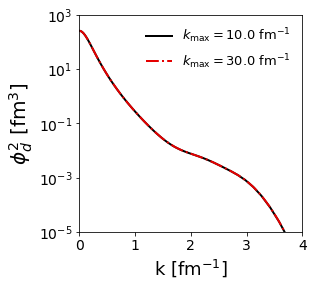
\includegraphics[clip,clip,width=0.6\textwidth]{momentum_distribution_test.png}%
    \caption{Deuteron momentum distributions from the EM N$^3$LO 500 MeV potential with two different momentum meshes: $k_{\rm max}=10$ and $30$ fm$^{-1}$.}
    \label{fig:momentum_distributions}
\end{figure*}
%


%%%%%%%%%%%%%%%%%%%%%%%%%%%%%%%%%%%%%%%%%%%%%%%%%%%%%%%%%%%%%%%%%%%%%%%%%
\section{Momentum projection operator}
\label{sec:momentum_projection_operator}


%
\begin{figure*}[tbh]
    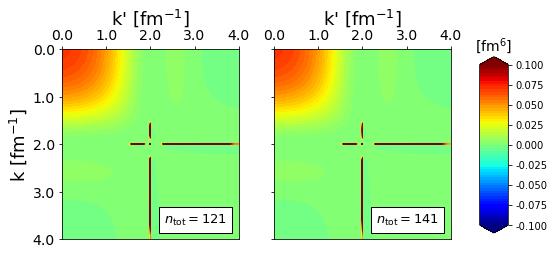
\includegraphics[clip,clip,width=0.9\textwidth]{momentum_projection_operator_test.png}%
    \caption{Momentum projection operators with $q=2$ fm$^{-1}$ under SRG transformations from EM N$^3$LO 500 MeV potential with two different momentum meshes: $N=121$ and $141$ where $k_{\rm max}=6$ and $k_{\rm mid}=2$ fm$^{-1}$. (This allows for the same value of $q=1.999$ fm$^{-1}$ in each mesh, so the initial operator is identical.) Here, we use the Wegner generator and set $\lambda=1.5$ fm$^{-1}$.}
    \label{fig:momentum_projection_operators}
\end{figure*}
%

In two-particle momentum-space, the momentum occupation operator $a^{\dagger}_q a_q$ is the same as the momentum projection operator $\ket{q} \bra{q}$.
We can connect the momentum projection operator to the normalization of the wave functions $\ket{\psi_{\alpha}}$.
We suppress the state index $\alpha$ in the following:
%
\begin{align}
    \label{eq:momentum_proj_operator_derivation}
    1 &= \bra{\psi} \ket{\psi} \nonumber \\
    &= \frac{2}{\pi} \int_0^{\infty} dq q^2 \bra{\psi} \ket{q} \bra{q} \ket{\psi} \nonumber \\
    &= (\frac{2}{\pi})^3 \int_0^{\infty} dq q^2 \int_0^{\infty} dk k^2 \int_0^{\infty} dk' k'^2 \bra{\psi} \ket{k} \mel{k}{a^{\dagger}_q a_q}{k'} \bra{k'} \ket{\psi} \nonumber \\
    &\approx (\frac{2}{\pi})^3 \sum_{n=1}^{N} w_n q_n^2 \sum_{i=1}^{N} w_i k_i^2 \sum_{j=1}^{N} w_j k_j^2 \bra{\psi} \ket{k_i} \mel{k_i}{a^{\dagger}_{q_n} a_{q_n}}{k_j} \bra{k_j} \ket{\psi} \nonumber \\
    &= \sum_{n=1}^{N} \sum_{i=1}^{N} \sum_{j=1}^{N} ( \sqrt{\frac{2 w_i}{\pi}} k_i \bra{\psi} \ket{k_i} ) ( \frac{2}{\pi} w_n q_n^2 \frac{2}{\pi} k_i k_j \sqrt{w_i w_j} \mel{k_i}{a^{\dagger}_{q_n} a_{q_n}}{k_j} ) ( \sqrt{\frac{2 w_j}{\pi}} k_j \bra{k_j} \ket{\psi} ) \nonumber \\
    &= \sum_{n=1}^{N} \sum_{i=1}^{N} \sum_{j=1}^{N} (\tilde{\psi_{\alpha}^*})_i \frac{2}{\pi} w_n q_n^2 ( \tilde{a}^{\dagger}_{q_n} \tilde{a}_{q_n})_{ij} (\tilde{\psi_{\alpha}})_j.
\end{align}
%
From this, we identify
%
\begin{align}
    \label{eq:momentum_proj_op_with_factors}
    (\tilde{a}^{\dagger}_{q_n} \tilde{a}_{q_n})_{ij} = \frac{\pi \delta_{ni} \delta_{nj}}{2 w_n q_n^2},
\end{align}
%
\begin{align}
    \label{eq:momentum_proj_op}
    \mel{k_i}{a^{\dagger}_{q_n} a_{q_n}}{k_j} = \frac{\pi (\tilde{a}^{\dagger}_{q_n} \tilde{a}_{q_n})_{ij}}{2 k_i k_j \sqrt{w_i w_j}}.
\end{align}
%


For the purposes of presentation, we want to plot mesh-independent results analogous to plotting mesh-independent potentials.
This concept should be generalized to \emph{any} operator.
Thus, we plot Eq.~\ref{eq:momentum_proj_op} to visualize the momentum projection operator.
In applying SRG transformations to this operator, use Eq.~\eqref{eq:momentum_proj_op_with_factors}, because the transformations are typically constructed out of the normalized eigenvectors of the initial and evolved Hamiltonians meaning the transformation matrix already includes the momenta and weights for ``integrating'' over $dk$ and $dk'$.
Figure \ref{fig:momentum_projection_operators} shows SRG-evolved momentum projection operators $\mel{k_i}{a^{\dagger}_{q_n} a_{q_n}}{k_j}_{\lambda}$ at $q=2$ fm$^{-1}$ and $\lambda=1.5$ fm$^{-1}$ for two different momentum meshes.


Let's do a sanity check by evaluating $\mel{\psi}{a^{\dagger}_q a_q}{\psi}=|\psi(q)|^2$. Note, this is the squared value of the wave function $\psi$ with momenta and weights divided out, evaluated at some momentum value $q$ where the units are fm$^3$.
In the following check, let $q$ also denote the index of the momentum value $q$ within the momentum array.
%
\begin{align}
    \label{eq:momentum_proj_check}
    \mel{\psi}{a^{\dagger}_q a_q}{\psi} &= (\frac{2}{\pi})^2 \int_0^{\infty} dk k^2 \int_0^{\infty} dk' k'^2 \bra{\psi} \ket{k} \mel{k}{a^{\dagger}_q a_q}{k'} \bra{k'} \ket{\psi} \nonumber \\
    &\approx (\frac{2}{\pi})^2 \sum_{i=1}^{N} w_i k_i^2 \sum_{j=1}^{N} w_j k_j^2 \bra{\psi} \ket{k_i} \mel{k_i}{a^{\dagger}_{q} a_{q}}{k_j} \bra{k_j} \ket{\psi} \nonumber \\
    &= (\frac{2}{\pi})^2 \sum_{i=1}^{N} w_i k_i^2 \sum_{j=1}^{N} w_j k_j^2 \bra{\psi} \ket{k_i} \frac{\pi^2 \delta_{ni} \delta_{nj}}{4 q_n^2 w_n k_i k_j \sqrt{w_i w_j}} \bra{k_j} \ket{\psi} \nonumber \\
    &= \bra{\psi} \ket{q} \bra{q} \ket{\psi} \nonumber \\
    &= |\psi(q)|^2.
\end{align}
%

\noindent{
\textbf{Alternative derivation of the momentum projection operator}
}


Let's start by defining the projection operator in Dirac notation for discrete states $\alpha$.
The states are orthogonal and satisfy the completeness relation
%
\begin{align}
    \label{eq:orthogonality}
    \bra{\alpha} \ket{\beta} = \delta_{\alpha \beta},
\end{align}
%
\begin{align}
    \label{eq:completeness}
    \mathbb{1} = \sum_{\alpha} \ket{\alpha} \bra{\alpha} \equiv \sum_{\alpha} P_{\alpha},
\end{align}
%
where $P_{\alpha} \equiv \ket{\alpha} \bra{\alpha}$ is the projection operator for the state $\alpha$.
We can expand any state $\ket{\psi}$ in terms of the states $\ket{\alpha}$,
%
\begin{align}
    \label{eq:expansion_of_psi}
    \ket{\psi} = \sum_{\alpha} \bra{\alpha} \ket{\psi} \ket{\alpha} = \sum_{\alpha} P_{\alpha} \ket{\psi}.
\end{align}
%
Matrix elements of the projection operator are given by
%
\begin{align}
    \label{eq:projection_operator}
    \mel{\beta}{P_{\alpha}}{\gamma} = \bra{\beta} \ket{\alpha} \bra{\alpha} \ket{\gamma} = \delta_{\beta \alpha} \delta_{\alpha \gamma},
\end{align}
%
where we used the orthogonality relation Eq.~\eqref{eq:orthogonality} in the last step.
We can make a consistency check with the projection operator $P_{\alpha}$ by using it to evaluate the normalization of the wave function,
%
\begin{align}
    \label{eq:normalization}
    \sum_{\alpha} \mel{\psi}{P_{\alpha}}{\psi} &= \sum_{\alpha} \sum_{\beta} \sum_{\gamma} \bra{\psi} \ket{\beta} \mel{\beta}{P_{\alpha}}{\gamma} \bra{\gamma} \ket{\psi} \nonumber \\
    &= \sum_{\alpha} \sum_{\beta} \sum_{\gamma} \bra{\psi} \ket{\beta} \bra{\beta} \ket{\alpha} \bra{\alpha} \ket{\gamma} \bra{\gamma} \ket{\psi} \nonumber \\
    &= \sum_{\alpha} \sum_{\beta} \sum_{\gamma} \bra{\psi} \ket{\beta} \delta_{\beta \alpha} \delta_{\alpha \gamma} \bra{\gamma} \ket{\psi} \nonumber \\
    &= \sum_{\alpha} \bra{\psi} \ket{\alpha} \bra{\alpha} \ket{\psi} \nonumber \\
    &= \bra{\psi} \ket{\psi}.
\end{align}
%


Now, let's do the same derivation but for two-particle partial-wave momentum-space with basis states $\ket{klm}$.
In this basis, the orthogonality condition is given by
%
\begin{align}
    \label{eq:orthogonality_ms}
    \bra{klm} \ket{k'l'm'} = \frac{\pi}{2kk'} \delta(k-k') \delta_{ll'} \delta_{mm'}.
\end{align}
%
(This can be verified by taking $\ket{k'l'm'}$ to both sides of Eq.~\eqref{eq:completeness_relation}.)
Likewise we can expand any state $\ket{\psi}$ using the completeness relation Eq.~\eqref{eq:completeness_relation},
%
\begin{align}
    \label{eq:expansion_of_psi_ms}
    \ket{\psi} = \frac{2}{\pi} \sum_{l,m} \int_0^{\infty} dk k^2 \bra{klm} \ket{\psi} \ket{klm} = \frac{2}{\pi} \sum_{l,m} \int_0^{\infty} dk k^2 P_{klm} \ket{\psi},
\end{align}
%
where $P_{klm} \equiv \ket{klm} \bra{klm}$.
Matrix elements of the projection operator are then
%
\begin{align}
    \label{eq:projection_operator_ms_1}
    \mel{klm}{P_{ql''m''}}{k'l'm'} &= \bra{klm} \ket{ql''m''} \bra{ql''m''} \ket{k'l'm'} \nonumber \\
    &= \frac{\pi}{2kq} \delta(k-q) \delta_{ll''} \delta_{mm''} \frac{\pi}{2qk'} \delta(q-k') \delta_{l''l'} \delta_{m''m'}.
\end{align}
%
If we fix the relative orbital angular momentum and projection to $l$ and $m$, respectively, we obtain
%
\begin{align}
    \label{eq:projection_operator_ms_2}
    \mel{k}{P_{q}}{k'} = \frac{\pi^2}{4q^2kk'} \delta(k-q) \delta(q-k'),
\end{align}
%
in agreement with Eqs.~\eqref{eq:momentum_proj_op_with_factors} and \eqref{eq:momentum_proj_op}.
(Note, this has not accounted for the ``discrete'' numerical problem.
Going one step further would introduce sums and weights instead of the integral over $dk$.)
The normalization check is very straight forward and proceeds in the same manner as Eq.~\eqref{eq:momentum_proj_operator_derivation}.
    

%%%%%%%%%%%%%%%%%%%%%%%%%%%%%%%%%%%%%%%%%%%%%%%%%%%%%%%%%%%%%%%%%%%%%%%%%
\section{Radius-squared operator}
\label{sec:radius_squared_operator}


In order to plot the $r^2$ operator in partial-wave momentum-space, we must change the operator from coordinate-space to partial-wave momentum-space.
Technically, we could make calculations with the $r^2$ operator fully in momentum-space where the operator involves derivatives $\frac{d}{dk}$ acting on a wave function.
However, we avoid this as the derivatives make it impossible to see the operator directly.
In coordinate-space, the operator is given by
%
\begin{align}
    \label{eq:r2_operator_coordinate_space}
    \mel{\mathbf{r}}{r^2}{\mathbf{r'}} = r^2 \delta(\mathbf{r}-\mathbf{r'}).
\end{align}
%
We can transform the operator to partial-wave momentum-space using
%
\begin{align}
    \label{eq:hankel_transformation}
    \bra{\mathbf{r}} \ket{klm} \equiv i^l j_l(kr) Y_{lm}(\Omega_r),
\end{align}
%
and the completeness relation in coordinate-space,
%
\begin{align}
    \label{eq:completeness_relation_coordinate_space}
    \mathbb{1} = \int d\mathbf{r} \ket{\mathbf{r}} \bra{\mathbf{r}},
\end{align}
%
(see Dirac QM2 for further details.)


Now we can isolate the radius-squared operator in momentum-space,
%
\begin{align}
    \label{eq:r2_operator_momentum_space_1}
    \mel{klm}{r^2}{k'l'm'} &= \int d\mathbf{r} \int d\mathbf{r'} \bra{klm} \ket{\mathbf{r}} \mel{\mathbf{r}}{r^2}{\mathbf{r'}} \bra{\mathbf{r'}} \ket{k'l'm'} \nonumber \\
    &= \int d\mathbf{r} \int d\mathbf{r'} [i^l j_l(kr) Y_{lm}(\Omega_r)]^* r^2 \delta(\mathbf{r}-\mathbf{r'}) [i^{l'} j_{l'}(k'r') Y_{l'm'}(\Omega_{r'})] \nonumber \\
    &= \int_0^{\infty} dr r^2 \int d\Omega_r (i^l)^* j_l(kr) Y_{lm}^*(\Omega_r) r^2 i^{l'} j_{l'}(k'r) Y_{l'm'}(\Omega_r) \nonumber \\
    &= \delta_{ll'} \delta_{mm'} (i^l)^* i^{l'} \int_0^{\infty} dr r^4 j_l(kr) j_{l'}(k'r),
\end{align}
%
where we have used the normalization of the spherical harmonic functions in the last step.
Rewriting Eq.~\eqref{eq:r2_operator_momentum_space_1} for the case $l=l'$ and $m=m'$ gives
%
\begin{align}
    \label{eq:r2_operator_momentum_space_2}
    \mel{k}{r^2}{k'}_{lm} = \int_0^{\infty} dr r^4 j_l(kr) j_{l}(k'r).
\end{align}
%
Then switching from a continuous to a discrete basis gives
%
\begin{align}
    \label{eq:r2_operator_momentum_space_3}
    \mel{k_i}{r^2}{k_j}_{lm} = \sum_{m=1}^M \Delta r r_m^4 j_l(k_i r_m) j_{l}(k_j r_m),
\end{align}
%
where we have a linearly spaced array of $r$ values where $dr \rightarrow \Delta r$ and $M$ is the number of values in the array.
Following the general convention from before, we define the operator with momenta and weights factored in,
%
\begin{align}
    \label{eq:r2_operator_momentum_space_with_factors}
    (\tilde{r}_{lm}^2)_{ij} \equiv \frac{2}{\pi} k_i k_j \sqrt{w_i w_j} \mel{k_i}{r^2}{k_j}_{lm}.
\end{align}
%
\begin{figure*}[tbh]
    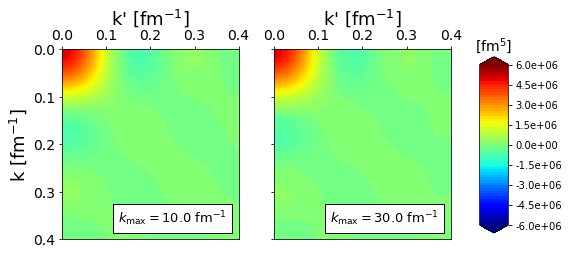
\includegraphics[clip,clip,width=0.9\textwidth]{r2_operator_test.png}%
    \caption{$r^2$ operators under SRG transformations from EM N$^3$LO 500 MeV potential with two different momentum meshes: $k_{\rm max}=10$ and $30$ fm$^{-1}$. Here, we use the Wegner generator and set $\lambda=1.5$ fm$^{-1}$.}
    \label{fig:r2_operators}
\end{figure*}
%

%%%%%%%%%%%%%%%%%%%%%%%%%%%%%%%%%%%%%%%%%%%%%%%%%%%%%%%%%%%%%%%%%%%%%%%%%


\bibliography{tropiano_bib}

\end{document}